\documentclass{article}
\usepackage{graphicx}
\usepackage{amsmath}

\begin{document}

    \title{Understanding the Dynamics of Human Questioning and Perception Over Time}
    \author{Kilian Lehn}
    \date{\today}
    \maketitle


    \section{Introduction}

    In this document, we present a model to investigate the dynamics of human questioning behavior and the development of understanding over a lifetime. Everything is interconnected through time and space, and human perception further adds independent variables to this complex reality. Our approach to examining this complexity is through the lens of categories of perception and understanding.


    \section{Perception, Understanding, and Their Dynamics}

    Humans perceive reality through various categories of perception. Over time, these perceptions evolve and form clusters of understanding. To truly assess the consistency of these perceptions, one would have to conduct a longitudinal study spanning a human's lifetime. Through such an investigation, we would be able to measure the perception space by means of multidimensional scaling, observing the rate of change in the aspects significant to the individual.

    However, it is essential to recognize that it is impossible to identify unknown schemes or mechanisms. This highlights the need to understand one's own cognitive structures. By identifying the boundaries of our mindset, we can challenge and transcend them. As stated by Einstein, our theories often determine our observations, and we tend to observe what confirms our theories, thereby reinforcing our beliefs.

    \clearpage


    \section{Questioning and Understanding: A Model}

    The described dynamics are based on two key assumptions:
    \begin{enumerate}
        \item We can understand the dynamics and mechanisms of the human mind's data processing to a certain extent when we compare it in two layers. The second layer is predicated on achieving the first layer, as it requires a broad understanding of personal questioning patterns:
        \begin{itemize}
            \item \textit{First Layer - Local to Global Perception of Own Questioning Patterns}: Questioning is a constant process. Reality aligns with it to a certain degree. Consequently, our personal reality is substantially shaped by the way we ask questions. This leads to the understanding that questioning is the independent variable and reality the dependent one. Thus, our prognoses are progressively fine-tuned, not to reality, but to the underlying patterns of how we question reality.
            \item \textit{Second Layer - Establishing Feedback Loops of Global Perception of Own Questioning Patterns to Reality}: Once a comprehensive understanding of personal questioning patterns has been achieved, we can then benchmark these against reality. However, we are limited by time. This means we have only a finite number of moments to align our abstractions against reality and discover the fundamental patterns of our questioning. As such, moments not spent questioning, not formulating prognoses, or not pushing the boundaries of our sense perceptions can be considered 'wasted' from the perspective of understanding development.
        \end{itemize}
    \end{enumerate}
    \label{sec:assumptions}


    \section{Implementation and Further Discussion}

    We propose a Python class \texttt{Person}, which allows to plot the formulated assumptions up until the second layer.


    \section{Mathematical Model}

    The frequency $F_t$ of questioning at time $t$ is modeled as an exponential decay process with an initial frequency $F_0$ and a rate of change $r_F$:

    \[
        F_t = F_0 \exp(-r_F t)
    \]

    With the understanding that an exponential increase in question quality and an exponential decrease in question frequency leads to a nonlinear progression of understanding, we model the level of understanding $U_t$ at time $t$ with an initial understanding $U_0$ and a rate of increase $r_U$ that is proportional to the product of the quality and frequency of questions:

    \[
        U_t = U_0 + r_U Q_t F_t
    \]

    Where $Q_t$ represents the quality of questions over time, which increases exponentially.

    \begin{figure}[ht]
        \centering
        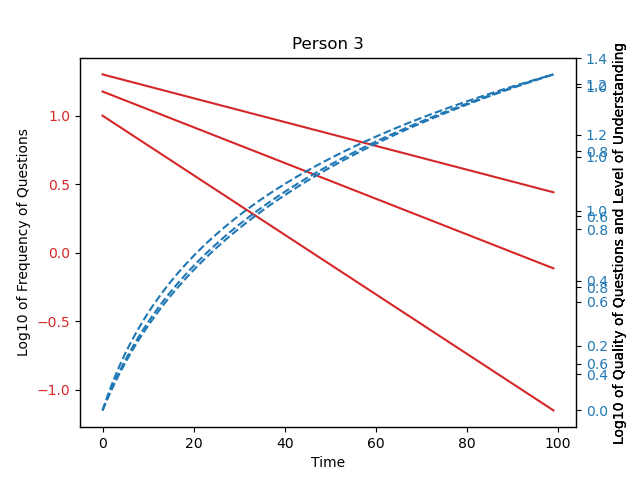
\includegraphics[width=0.7\textwidth]{combined_plot.png}
        \caption{Combined Plot of Persons}
        \label{fig:combinedplot}
    \end{figure}


    \section{Discussion}

    The model provides a highly simplified representation of the complex processes of human questioning and understanding development. Although it does not capture all the nuances of these processes, it offers a starting point for understanding their dynamics and how they might change under different conditions.

    \subsection{Person 1}

    Person 1, who experiences the strongest increase in the quality of questions and level of understanding, sees the largest decrease in the frequency of questions over time. This is based on the correlation that an increase in the quality of questions and level of understanding causes a decrease in the frequency of questions. A similar pattern can be observed for Person 2 and Person 3, though the changes are less pronounced.

    \subsection{Person 2}

    Person 2 exhibits a moderate increase in the quality of questions and level of understanding, resulting in a gradual decrease in the frequency of questions over time. The changes in frequency, quality, and understanding are less pronounced compared to Person 1.

    \subsection{Person 3}

    Person 3 shows a relatively slower increase in the quality of questions and level of understanding. As a result, the decrease in the frequency of questions over time is less significant compared to Person 1 and Person 2.


    \section{Perception, Time, and the Pursuit of Eternity}

    In the pursuit of understanding, there comes a time when the average used categories of perception align perfectly with the perception-patterns of reality. This is the moment when our known categories are sufficient to comprehend the moment entirely. This is the point where the second layer mentioned in Section~\ref{sec:assumptions} comes into play. Only when the global trends of our questioning patterns are observable, then we can start to benchmark them against reality.

    Here just for getting across the concept of a global trend map of the questioning patterns (see code and you will see, that its really just that):

    \begin{figure}[ht]
        \centering
        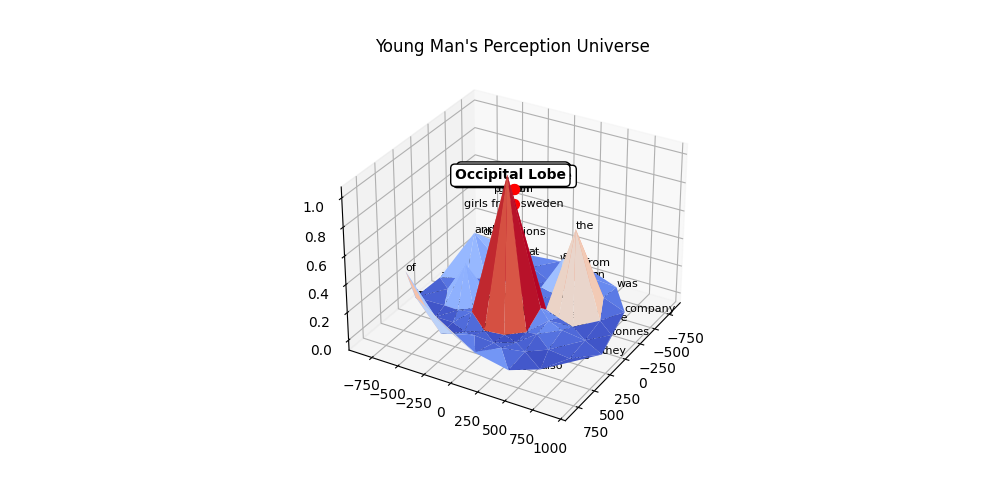
\includegraphics[width=0.7\textwidth]{3d_plot.png}
        \caption{3D Plot}
        \label{fig:3dplot}
    \end{figure}


    \section{Conclusion}

    In a life where an individual fails to recognize patterns and dynamics (single-case-life), each day unfolds as a new exciting adventure, and time becomes a precious commodity. Conversely, in a life where past experiences are recognized in latent mechanisms and dynamics (abstract-case-life), time loses importance as one can anticipate what has happened and what will happen - time becomes eternal.

\end{document}
